 \documentclass[11pt]{article}
 % TODO Minimumschaltung + Funktion drauf

\usepackage{graphicx}
\usepackage[utf8]{inputenc}
\usepackage{amsmath}
\usepackage[top=1in, bottom=1.25in, left=1.25cm, right=1.25in]{geometry}


\begin{document}

\begin{minipage}{0.33\textwidth}

\underline{\textbf{Grundformeln:}}\\
WS: $R = \frac{U}{I} = \frac{\rho \cdot l}{A}$; $[R] = 1\frac{V}{A} =1 \Omega$\\
Leitwert: $G = \frac{1}{R}$\\
\textbf{Maschensatz: $\mathbf{\sum U_i = 0}$\\}
\textbf{Knotensatz: $\mathbf{\sum I_i = 0}$\\}
Reihe WS: $R_{ges} = \sum R_i$\\
Parallel WS: $\frac{1}{R_{ges}} = \sum \frac{1}{R_i}$\\
\phantom{ss} Spezialfall: $R_{ges} = \frac{R_1 \cdot R_2}{R1+R2} $\\
\textbf{U-Teiler: $\mathbf{\frac{U_1}{U_2} = \frac{R_1}{R_2}\Leftrightarrow I_1 = I_2}$\\}
\textbf{I-Teiler: $\mathbf{\frac{I_1}{I_2} = \frac{R_2}{R_1}\Leftrightarrow U_1 = U_2}$\\}
Leistung: $P =U \cdot I = \frac{U^2}{R} = I^2 \cdot R $ \\
\phantom{ssssssssss} $[P] = 1V \cdot A =1 W$\\
Kein Strom $\Rightarrow$ U in Masche gleich!\\
U zu Masse $\Rightarrow$ alles danach drin

\underline{\textbf{Kondensator:}}\\
Kapazität: $C = \frac{Q}{U} = \frac{\varepsilon \cdot A }{d},$\\
\phantom{ssssssssssii} $[C]=1F$\\
Ladung: $Q = \int_{t_0}^t i(\tau) d\tau + q_0$\\
\phantom{sssssssis} $\stackrel{homogen}{=} I \cdot t$\\
\phantom{ssssssssssii} $[q]=1C$\\
Spannung: $U = \frac{Q}{C}$\\
Kond. parallel: $C_{ges} = C_1 + C_2$\\
Kond. in Reihe: $C_{ges} = C_1 || C_2$\\
Kond. in Reihe: $Q_1 = Q_2 = Q_{12}$\\

$u_c(t) = u_c(\infty) + (u_{pre} - u_c(\infty)) \cdot e^{-\frac{t-t_0}{\tau}}$\\
Wenn WS dazu, dann V-Teiler\\
$[k] = 1V$\\
Str.q: $U = \frac{Q}{C} = \frac{I_q \cdot (t-t_0)}{C} + U_c(t_0)$\\
\phantom{sss} ,Kennlinie linear\\
\textbf{2}Zeitkonst.: $\tau = R \cdot C;[\tau] = 1s$\\
\phantom{ss}falls WS in Reihe $\Rightarrow$ parallel\\
$t =\frac{T}{2} = \frac{1}{2f}$\\
Zeit Auf-/Entlanden: $t = 3\tau$\\

"einge." $\Rightarrow i_C = C \cdot \frac{dU_c}{dt} = 0$\\
\phantom{sss} $\Rightarrow U_x = 0 \Rightarrow U_Y = U_B$

Arbeit(=Energie): $W = \int_0^\infty P dt$\\
\phantom{sssssssss} $= \frac{U_b^2 \cdot C}{2} $\\
\phantom{sssssssss} $= [W] = 1J $\\
$W_{Zyklus} = W_a + W_e$\\
$\overline{P} = \frac{W_{Zyklus}}{T}$\\
Tiefpass: Oben R, Mitte C, Integrator\\
HP: Kennl.$U_A$ seltsam,$U_E$ normal
\end{minipage}%
~~~~~~~
\begin{minipage}{0.33\textwidth}

\underline{\textbf{Felder:}}\\
Stromdichte: $S=\frac{I}{A}$\\
Feldstärke: $E=\frac{S}{\kappa}$\\
Spannungsabfall: $U=E \cdot l$\\
Pot.: $\varphi (x)= \int_x^0 E(s)ds + \varphi(0)$\\
Stromstärke: $I = \oint H ds = H \cdot 2\pi r$\\
Mag.Feldstr.: $H = \frac{I}{2\pi d}, [H] = 1\frac{A}{m}$\\
Kraft pro Leitungslänge:\\
\phantom{ss} $F=Q \cdot v \cdot B, [F] = 1N$\\
Ladung pro mm: $Q = \rho \cdot V$\\
$e^-$, Drift-Gesch.: $v = \frac{S}{\rho}, [v] = 1\frac{m}{s}$\\
Flussdichte: $B=\mu \cdot H, [B] = 1 \frac{Vs}{m^2}$\\
 
 \underline{\textbf{(Koaxial-)Leitungen}}:\\
$R_W = \sqrt{\frac{L'}{C'}}$\\
    \phantom{sssi} $=\frac{\sqrt{\mu_R} \cdot ln(\frac{d_a}{d_i})}{2c_0 \cdot \pi \cdot \epsilon_0 \cdot \sqrt{\epsilon_R}}$\\
$C = \frac{1}{\sqrt{L' \cdot C'}} = \frac{c_0}{\sqrt{\epsilon_r \cdot \mu_s}}$\\
$C' = \frac{2\pi \epsilon_0 \epsilon_r \cdot s}{ln(\frac{d_a}{d_i})}$ = $\frac{C}{l}$\\
$L' = \frac{\sqrt{\epsilon_r \mu_r}}{c_0 \cdot \sqrt{C'}}$\\
$X' = \frac{X}{l}$\\

$k_0 = \frac{R_w}{R_w + R_i} $\\
$r_a = \frac{R_a - R_w}{R_a + R_w} $\\
$k_a = 1 + r_a = k_1$\\
$R_w \hat{=}$ WS der Leitung\\
$R_i \hat{=}$ WS vor der Leitung\\
$R_a \hat{=}$ WS nach der Leitung\\
$U_q == U_i$\\
$t_i \hat{=}$ High-Zeit\\
Reflexion: $U_r(l,t) = r_a \cdot U_k(l,t)$\\
Anfang: $U_k(0,t)=k_0 \cdot U_{q}(t)$\\
Mitte/Ende:\\
\phantom{ss} $U_k(x,t)= k_0 \cdot U_{q}(t-\Delta t)$\\
\phantom{sss}$\Delta t = \frac{l}{c} = \frac{l}{\lambda f}$\\
Auskoppeln Gatter:\\
\phantom{ss} $U_1(t) = k_a \cdot U_k(x,t) $\\
\phantom{sssssssiiii}$= k_a\cdot k_0 \cdot U_q(t-\Delta t)$\\
V Ende Leitung: $u_a = k_0 \cdot k_a \cdot u_q$\\

LW-Leitung: $\alpha = \frac{L_P}{l}; [\alpha] = 1 \frac{dB}{m}$\\
Lichtleistung: $L_P = 10 \cdot lg\frac{P_e}{P_a} dB$\\
\phantom{sssssississsssss} $L_P = l \cdot \alpha$\\
\phantom{sssssississsssss}$ [L_P] = 1dB$\\



\end{minipage}%
~~~~~~
\begin{minipage}{0.33\textwidth}
\underline{\textbf{Operationsverstärker:}}\\
$V_D = \infty I_P=I_N=R_D=U_D=V_G=R_a=0$\\
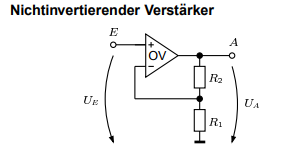
\includegraphics[scale=0.40]{NIOV.png}
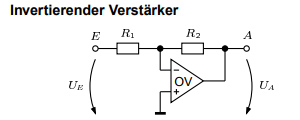
\includegraphics[scale=0.40]{IOV.png}
$U_D = 0 \Rightarrow I_N = 0, U_N = 0$\\

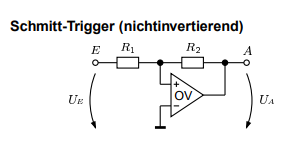
\includegraphics[scale=0.40]{NISTOV.png}\\
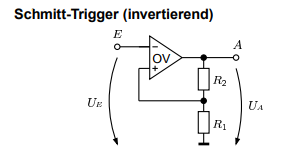
\includegraphics[scale=0.40]{ISTOV.png}\\
Umschalt.:$U_D = 0 \Rightarrow U_G = U_{SP}$\\
$U_A \in \{U_B,0\}$\\
$U_D = 0 = U_P - U_{E_{HL}}$\\
\phantom{sssi}$\Rightarrow U_{E_{HL}} = \frac{U_{A_{max}} \cdot R_1}{R_1 + R_2}$\\
$U_D = 0 = U_P - U_{E_{LH}}$\\
\phantom{sssi}$\Rightarrow U_{E_{LH}}= \frac{ U_{A_{min}} \cdot R_1}{R_1 + R_2}$\\
Diode: $\Rightarrow U_{E_{LH}} = 0$\\
Schalthysterese:\\
\phantom{sssssi} $H = |U_{E_{HL}} - U_{E_{LH}}|$\\
z.B. V Low-High: $\Rightarrow U_G = U_{SP}, U_A=L$

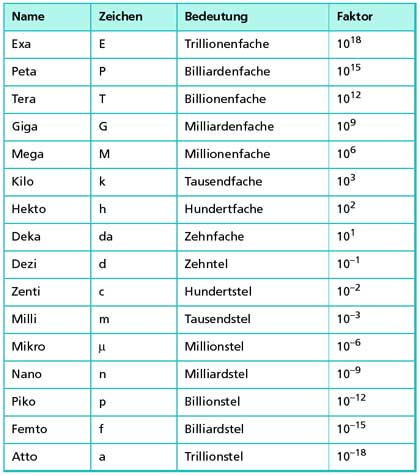
\includegraphics[scale=0.40]{Zehnerpotenzen.jpg}

\end{minipage}%

\newpage

\begin{minipage}{0.33\textwidth}
\vspace{-1cm}
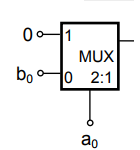
\includegraphics[scale=0.40]{Mult.png}\\
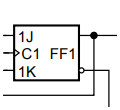
\includegraphics[scale=0.40]{FF.png}\\

\underline{\textbf{Diode:}}\\
Gesperrt: $U_D < U_{F_0}$\\
Leitend: $\Rightarrow U_D = U_{F_0}$\\
D sperrt: $\Rightarrow I_D(raus) = (-I_S|0)$\\
WS-Frei

\underline{\textbf{Transistor:}}\\
$I_G \stackrel{!}{=} 0A$\\

n-Kanal:\\
- Pfeil auf Gate\\
- Sperrt: $U_{GS} < U_{th}$\\
- Leitet: $\Rightarrow U_{DS} \geq 0$\\
\phantom{sssssiisi} $ (\Rightarrow U_D > 0, U_S = 0)$\\
\phantom{sssssiisssi}$\Rightarrow I_D$(in D rein) $\geq 0$\\
\[I_{D_N} = \left\{
  \begin{array}{ll}
      0 & U_{GS} < U_{th}~$sperrt$\\
        \frac{1}{2} \cdot \beta \cdot(U_{GS} - U_{th})^2  \ & U_{DS} \ge U_{GS} - U_{th}$~pinch-off (evnt. noch 2. Gl aus MS/KS)$\\
        \beta \cdot((U_{GS} - U_{th}) \cdot U_{DS} - \frac{1}{2} \cdot U_{DS}^2)  \ & U_{DS} \leq U_{GS} - U_{th}$~aktiv (evnt. noch 2. Gl aus MS/KS)$\\
  \end{array}
\right.
\]

p-Kanal:\\
- Pfeil von Gate weg\\
- Sperrt: $U_{GS} > U_{th}$\\
- Leitet: $\Rightarrow U_{DS} \leq 0$\\
\phantom{ssssisisssi}$\Rightarrow I_D \leq 0$\\
Wo Source-Drain durch Pot.\\
NMOS hat nur nicht-negierte Literale und 1 Negation über kompletter Formel\\
PMOS hat nur negierte Literale\\
CMOS: komp. NMOS und PMOS Teile\\
$+$F. $\Rightarrow$ Parallelschaltung\\
$\mathbf{\cdot} \Rightarrow$ Reihenschaltung\\
\end{minipage}
~~~~~~~
\begin{minipage}{0.33\textwidth}


\underline{\textbf{Logik:}}\\
KDNF: Mint.(=1) $\Rightarrow e1e2e3 + ...\overline{0}$\\
KKNF:Maxt.(=0) $, (a+b+c) \cdot ...\overline{1}$\\
KV-Diagramme:\\ 
\textbf{3,4 Block Drehen}\\
Gray C., Rechtecke, übers. OK.\\
Gray C:$(\overline{A} \overline{B}), (\overline{A}B), (AB), (A\overline{B})$\\
min. DNF: 1en Verbinden\\
min. KNF: 0en, alle Var neg.\\
logische Fkt.:$F = \overline{AB} \Rightarrow $ NAND
log./Schalt-Verknüpfung:$y = \overline{AB} $\\
Nur NAND $\Rightarrow$ 2 Nega., keine +, 1N über ganzer Formel\\
$\overline{y}$ = NMOS\\
$\overline{NMOS} \rightarrow$ y = PMOS\\


\underline{\textbf{Multiplexer:}}\\
OBDD: Nutze Shannon(0en 1en\\
Ebenef(x)=Eb.Baum=Eb. Mult.\\

\vspace{3cm}
\underline{\textbf{Flip-Flop:}}\\
Zeitsteuerung:\\ ((1)$|$(2)takt(zustands)$|$(flanken))\\$|$(N. takt) - gesteuertes FF\\
$>$ Takt$\Rightarrow$ steig. TF\\
$\rlap{o}{>}$ Takt$\Rightarrow$ fall. TF\\
Datensteuerung:\\ Delay, Toggle(1E), RS, JK (2E)\\
MS-FF: $c_M=0,c_S=1 \Rightarrow$ +Fl.\\
J=S; K=R; 1,1 = Inv.\\
NAND: J-K:4, R-S:2,\\
Trans.: NAND: 4, D-FF: 14\\



\end{minipage}
~~~~~~~
\begin{minipage}{0.33\textwidth}

\underline{\textbf{Arten von Automaten:}}\\
- Mealy: \textbf{A}usgang hängt von \textbf{E}ingang und Zustand \textbf{Q} ab \\
- Moore: A hängt nur von Q ab \\
- Autonom: Kein E \\
- Asynchron: Kein Takt \\
- Flankengest. Oft Master-Slave \\

\underline{\textbf{Synthese}}\\
- Zustandsgraph $\Rightarrow$ ZF-AFT: Kenne Q, Q+ $\Rightarrow$ Wie FF's schalten

-11.6, 11.7: Graph $\Rightarrow$ Kodierung Zustände $\Rightarrow$ ZT+AT $\Rightarrow$ Schaltung
\vspace{5cm}

\underline{\textbf{Zustandsgraph:}}\\
- Ist im Prinzip totaler DFA\\
- Evnt. Startzustand\\
- K's(BZ-Code E's) als Zustände\\
- Code getakt. Ausgänge als BZ\\
- schreibe Code an jeden Zustand\\
- Ungetakt. Ausgänge an Pfeile\\
- Belegung der Eingänge an Pfeil\\

\underline{\textbf{One Hot Kodierung:}}\\
Für jeden Zustand genau ein FF an. Falls (0,0,0,...) Startzustand, dann muss FF0 immer 1 sein, außer wenn Zustand 0 ist, dann ist alles 0
\end{minipage}%

\vspace*{-0.3 cm}
\underline{\textbf{Arten von Tabellen:}}\\
- WW-Tabelle hat Eingänge und Ausgänge berechnet\\
- ZF-Tabelle hat Eingänge, Zustand(Q) $|$ und Folgezustand (Q+)\\
- ZÜ-Tabelle hat Zustand $\rightarrow$ Folgezustand(Q+) $|$ Eingänge\\
-ZF+AT: Code der Q's ohne E(K),E's, Zustände(Q), FF-E(J,K) $|$, FolgeZ(Q+), Ausgänge\textbf{!Gegenw.!},K+\\
\phantom{ss} J,K aus Formeln, Q+ aus J,K

\end{document}
